
\section{Additional notes}

\subsection{Language to Number Translation Tasks}

In the NALU paper, they include a ``Language to Number Translation Tasks'' that appears to perform multiplication, by applying a recurrent NALU. However, after contracting the authors this turns out not to be the case.

\begin{itemize}
\item Question: In 4.3, how big is the embedding layer output dimensionality?\\ Answer: From memory - i think it was 256.
\item Question: In 4.3, how big is the LSTM layer output dimensionality?\\ Answer: From memory - I think it was 10 (small)
\item Question: In 4.3, what output and input activation does the LSTM layer have, tanh? \\ Answer: It uses the standard LSTM construction - default in Tensorflow.
\item Question: In 4.3, is the Linear/NAC/NALU layer only used for the final element in the sequence? See diagram.\\ Answer: Correct.
\end{itemize}

\begin{figure}[h]
\centering
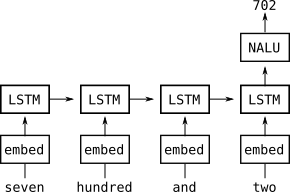
\includegraphics[scale=0.5]{graphics/language-to-numbers.png}
\caption{Diagram included in the email.} 
\end{figure}

Based on these answers, we don't believe ``Language to Number Translation Tasks'' tests multiplication in any meaningful way. There is nothing inherently wrong in that, as \citet{trask-nalu} don't state this explicitly either, we just wish to clarify this.

Our reasoning is that, an embedding of 256, is more than enough to fully describe every single token, keep in mind there are only 29 tokens in total. As such there is no reason why an LSTM layer wouldn't be able to solve this on its own (a simplified LSTM solving this task is seen in \eqref{eq:langauge-to-numbers-lstm}). Although, due to the non-linear activations, that are undesired in this case, the LSTM would need to downscale the values 0-1000 to be in the linear range of $\tanh(\cdot)$, and there would need to be final layer that upscales to 0-1000. We believe that the NALU layer serves this purpose and thus does not have any value in terms of arithmetics.

\begin{equation}
\begin{aligned}
h_t &= &h_{t-1}\ \cdot\ &f_t &&+ &\tilde{h}_{t}\ \ \cdot\ &i_t \\
h_t &= &\begin{bmatrix}
 h_{t-1} \\
 0 \\
 0
\end{bmatrix} &\left(I(x_t = \texttt{100})\begin{bmatrix}100 \\ 1 \\ 1\end{bmatrix}\right)\ &&+ &\begin{bmatrix}
 0 \\
 h_{t-1} \\
 x_t
\end{bmatrix} &\left(I(x_t \not= \texttt{100})\begin{bmatrix}100 \\ 1 \\ 1\end{bmatrix}\right)
\end{aligned}
\label{eq:langauge-to-numbers-lstm}
\end{equation}
